\documentclass[../../main.tex]{subfiles}


\begin{document}

\subsection*{(a)}
The following screenshots show the process used for 4a). A minimum support count of 250 was specified in the task. At a dataset size of 4982 this equals a minimum support of $\frac{250}{4982}=0.05$\\
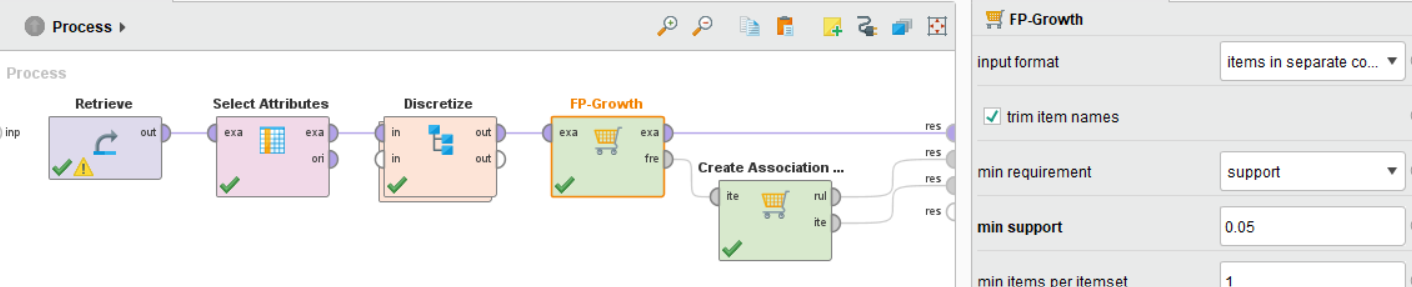
\includegraphics[width=\textwidth]{img/QUESTION_4a_PROCESS_overview.png}
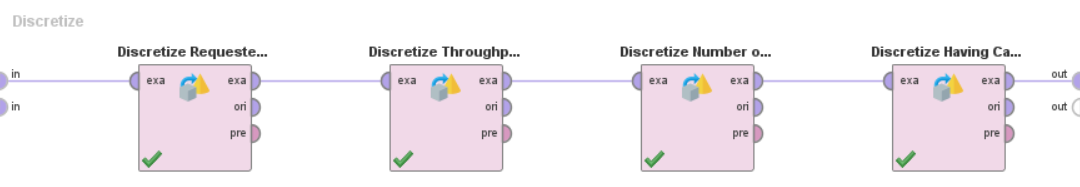
\includegraphics[width=\textwidth]{img/QUESTION_4a_PROCESS_discretize.png}
138 association rules were found at a minimum confidence of 0.8, the top 10 in confidence can be seen below:\\
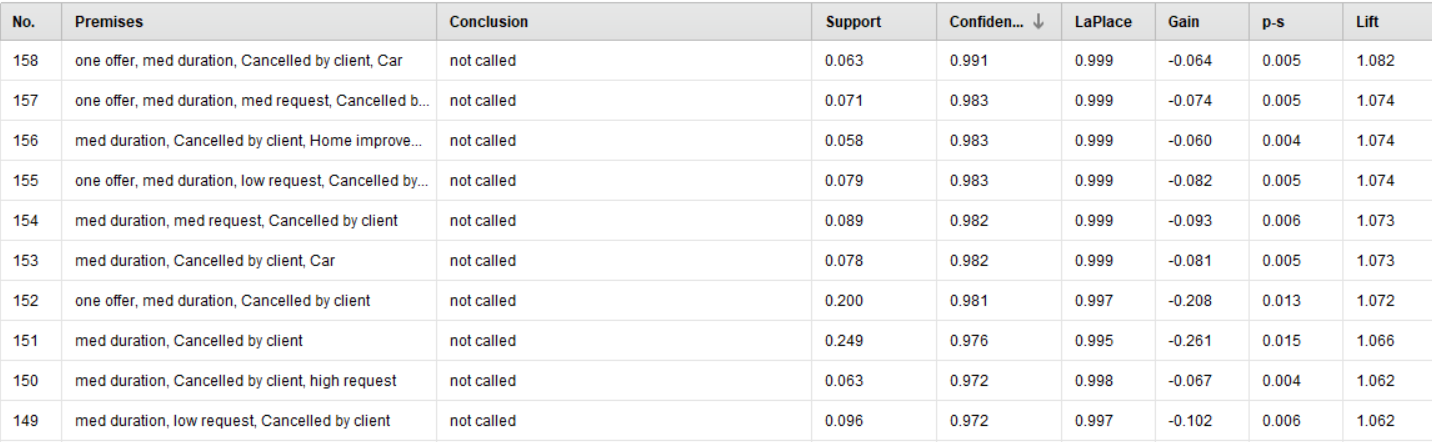
\includegraphics[width=\textwidth]{img/QUESTION_4a_association_rules.png}

\subsection*{(b)}
The conclusion with the highest confidence (0.991) states that if there is a car loan with one offer and a medium throughput time that gets cancelled by the client, the client likely doesn't call to complete the application 


\end{document}